\subsection{Motors} \label{analysisMotors}
In this subsection, a closer look at the different options of motors will be looked into. Since the NXT platform has been chosen it leaves roughly 14 motors to choose from\cite{}.

As given from the requirements we will need the bus to drive forward, stop and turn to both sides. To simplify, two motors will be chosen, one for each task. 

\begin{itemize}
    \item Driving Motor
    \item Turning Motor (servo only choice?)
\end{itemize}

To make sure not too much time is used on choosing motors by preforming test om them all. Data from other tests are used as guidelines, to pick out the motors. and our own tests will be preformed on these. 

\textbf{Driving Motor}
Choosing the best suited driving motor is important since it gives the bus the functionality of driving forward and stopping, and therefor needs to be able to both carry the weight of the bus, and still keep an constant speed.

From all the test preformed by ??\cite{}, only five seem to have a torque over 10N.cm. This spec is important since it shows how much work it can produce, however the speed of the work is determined by the rotation speed. Both of these go in hand, to find what motor can provide the best performance.

In table \ref{motorTable} the five motors can be seen with corresponding rotation speed and torque. From the table we can calculate ??, and find the best suited motor.


\begin{table}[H]
\centering
\begin{tabular}{|l|l|l|l|l|l|}
\hline
9V supply               & \textbf{\begin{tabular}[c]{@{}l@{}}Electric RC Race \\ Buggy Motor\end{tabular}} & \textbf{\begin{tabular}[c]{@{}l@{}}NXT Servo \\ Motor\end{tabular}} & \textbf{PF Medium} & \textbf{PF XL} & \textbf{PF Large} \\ 
\hline
\textbf{Rotation speed} & 1700 rpm/ 1240 rpm & 170 rpm & 405 rpm & 220 rpm & 390 rpm \\ 
\hline
\textbf{Stalled torque} & 14 N.cm & 50 N.cm & 11 N.cm & 40 N.cm & 18 N.cm \\ 
\hline
\end{tabular}
\caption{Comparison table of different motors compatible with LEGO NXT.}
\label{motorTable}
\end{table}


% Note Buggy Motor May need to much power to work with NXT, and will need EV3?. + Kræver converter kabel, da den er byggede til old brick



%http://www.philohome.com/motors/motorcomp.htm
%http://www.philohome.com/nxtmotor/nxtmotor.htm


\textbf{Turning Motor}






















%In this subsection, we will take a closer look at the motor. Since we chose the NXT as our platform there is only one option for our motor: the NXT motor.

% The motor takes PWM as input for controlling the speed; returns the completed rotations and degrees of the next rotation.

% The motor is supplied by a 9 V source. It's stalled torque is 50 N.cm, and it's stalled current is 2 A. The motor has a weight of 80g. Its maximum rotations per minute are 170, and its no-load current is 60 mA.\cite{motors}

% \begin{figure}[!ht]
%     \centering
% 	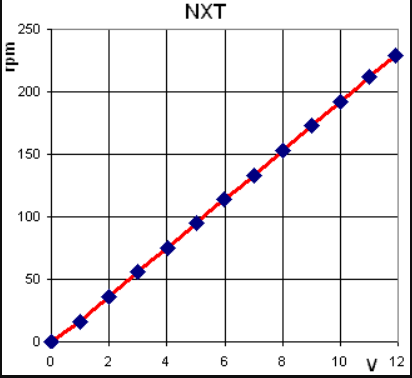
\includegraphics[width=0.7\textwidth]{Images/Analysis/nxtmotor.PNG}
%     \caption{Graph of rotations per minute as a function of voltage.\cite{motors}}
%     \label{fig:nxtmotor}
% \end{figure}